% !TEX root = ../../../Masterthesis.tex
\section{Enterprise Clears Moorings}
\begin{figure}[h!]
\center
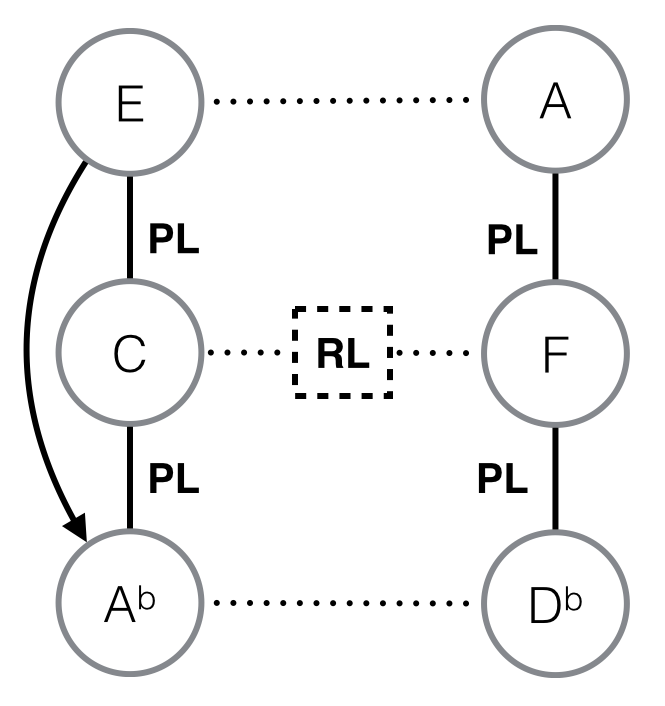
\includegraphics[width=0.6\linewidth]{ST2_Enterprise_PL}
	\caption{ST 2: Enterprise Clears Moorings, PL network}
	\label{ST2_Enterprise_PL}
	\setfloatalignment{b}
\end{figure}

\noindent The cue starts with an exterior shot of the Enterprise. Horner introduces a lydian inspired, slow and majestic theme as the Enterprise lights her external light buoys, preparing to leave the space dock. 

As soon as Kirk and Dr. McCoy enters the bridge, military snare drums and Horner's Star Trek theme plays over a G pedal. Woodwinds and wind chimes provide some lydian glitter just as the theme plays again. Spock is the Captain of the Enterprise and is seen overseeing the final preparations. The theme relies heavily on the mixolydian \flat6 scale\footnote{\keyboard{one=C,two=D,three=E,four=F,five=G,six=Giss,seven=Aiss,}\\Mixolydian \flat6: \textit{pc} [0,2,4,5,7,8,T]} and with it provides the harmonic backdrop.

\textbf{m.18-19} provides a section of \textit{parallel harmonic displacement}\footnote{Not unlike what we find in jazz big band traditions, where they are known as \textit{block chords} or \textit{chorale style harmony}.} seemingly unprovoked. It might be a mimicking of Spock, the half human and half Vulcan who is famous for his logic and lack of emotion; though this is pure speculation. In any case, it works as a transition and modulation for the Star Trek theme, now in F, and with an F pedal point until \textbf{m.29}.  

Figure \ref{ST2_Enterprise_PL} is a overview of the way Horner uses major thirds as a harmonic roadmap and has been the rule until now. Spock asks Lt. Saavik if she has ever before piloted a starship from the space dock. As she replies, Horner switches to a wondrous feeling \acf{MTTP} and hence makes use of his other harmonic road map, the RPRP network, as seen in figure \ref{ST2_Enterprise_RPRP}.

\begin{figure}
\center
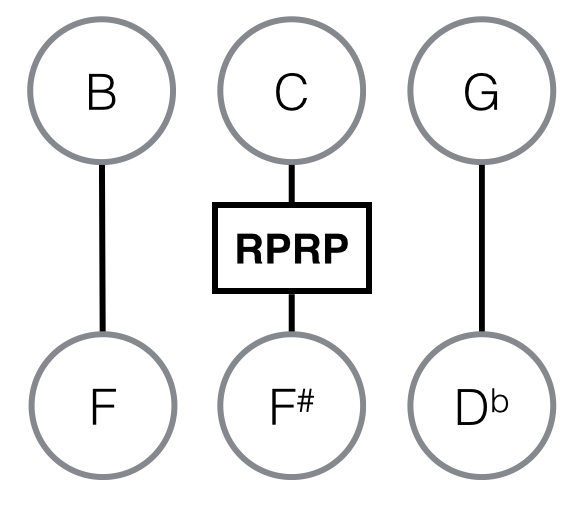
\includegraphics[width=0.6\linewidth]{ST2_Enterprise_RPRP}
	\caption{ST 2: Enterprise Clears Moorings, RPRP network}
	\label{ST2_Enterprise_RPRP}
	\setfloatalignment{b}
\end{figure}

Lt. Saavik accepts the challenge, which is followed by the main theme, and walks to the captain's chair. When walking Horner introduces a theme in A (\textbf{m.29}) which is lydian and familiar in tonality just as the theme in the beginning of the cue; however, this is not a theme but more for providing a sense of wonderment. 

Kirk is obviously nervous as Spock orders Lt. Saavik to take the ship out. The Star Trek theme modulates to D and sounds one last time before an accelerando and crescendo raises the excitement, along with Kirk, and hits the point of the Enterprise departing. Horner uses a variation of the sextuplet theme used in the Main Titles. The flurry of notes is backed up by a rising G lydian scale in the lower brass. After another \textbf{RPRP}, Horner revisits the Main Titles more, or less, exactly. From letter \textbf{I}, Horner has displaced the melody by one beat per what he did during the Main Titles. The chord structure Horner uses are major chords over the E minor scale (figure \ref{ST2_Enterprise_eminor}).

\begin{marginfigure}
%\center
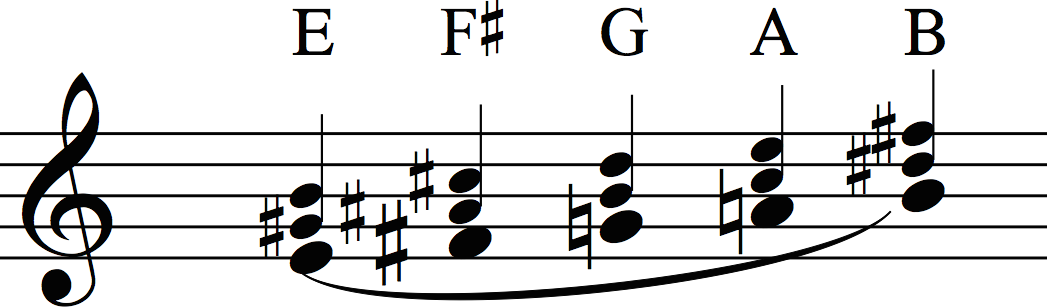
\includegraphics[width=\linewidth]{ST2_Enterprise_eminor}
	\caption{ST 2: Enterprise Clears Moorings, Major Chords over the E Minor Scale}
	\label{ST2_Enterprise_eminor}
	\setfloatalignment{b}
\end{marginfigure}

From \textbf{m.67} we return to the bridge and the music turns ominous. Descending and arpeggiated \(B^{(\sharp5)}\)'s with a quite energetic \(\hat{3}\) as the root. As with Spock, this seems unmotivated until one considers that working on a spaceship can be quite hazardous. The same descending pattern modulates up a fourth and is now joined by a fanfare that builds until Enterprise enters warp speed where Horner's music does exactly the same. There is a tiny tail where a major sixth is repeated, but the film cuts to a shot of a dark space station and the music turns to a flat 6, perhaps, making a prediction on its future.

%-----------------------------------------------------------------------------
% PDF
%-----------------------------------------------------------------------------
\clearpage
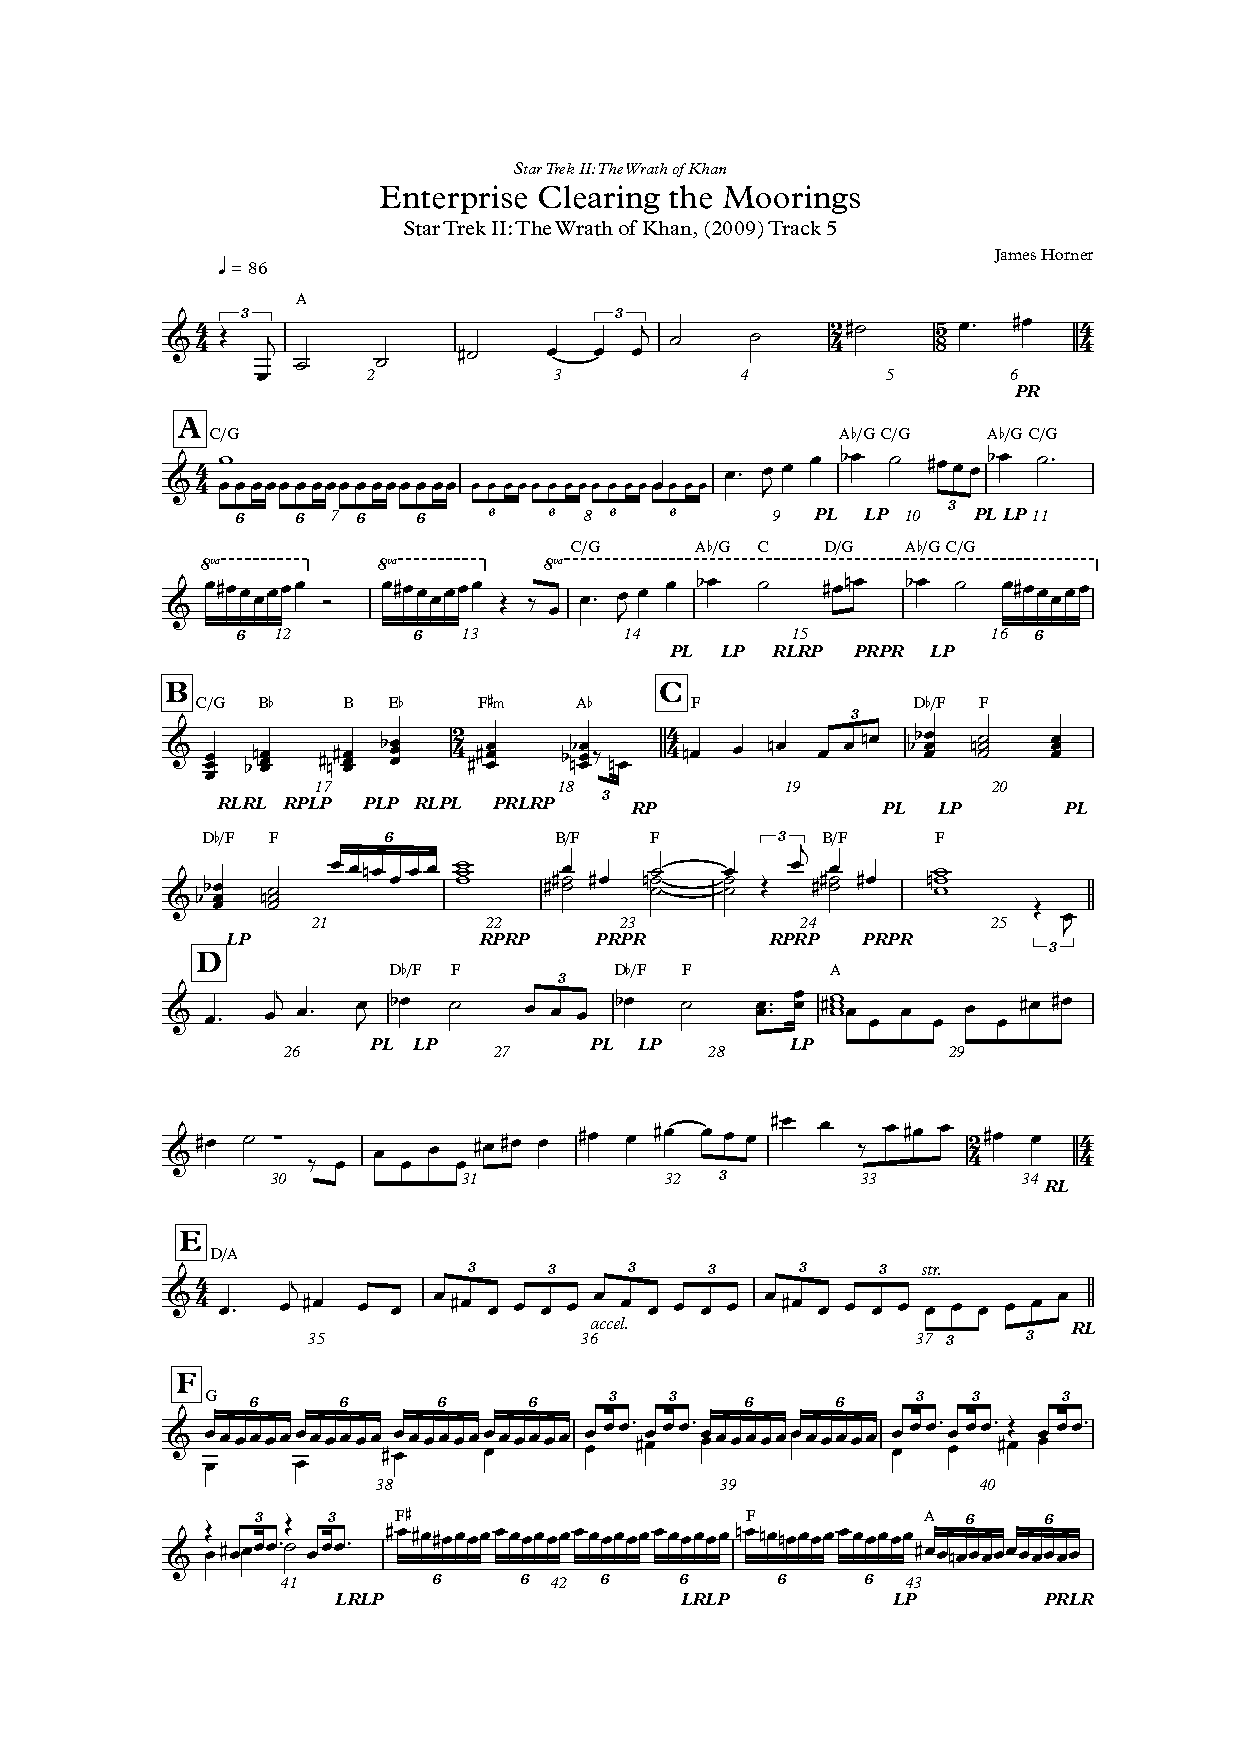
\includepdf[pages=-,pagecommand=\thispagestyle{fancy}]{pdf/st2/ST2_Enterprise_Clears_Moorings.pdf}

% Reviewed